% Provenance (never printed): old premiere S material on the lithosphere and the
% asthenosphere (chemical and mechanical layers, the low-velocity zone, the
% geotherm, isostasy); see sources/book2/PROVENANCE.md. S speeds from
% figdata/grade-11/prem_profiles.py (part upper), the geotherm and the solidus
% from geotherm_solidus.py, the elevations from hypsometry.py (ETOPO1).
% Glacial rebound belongs to g12; lithostatic pressure (term) to g12.
\chapter{स्थलमंडल और दुर्बलतामंडल}\label{ch:g11:lithosphere-asthenosphere}

हिमशैल का नौ-दशमांश भाग जल के नीचे रहता है: बर्फ़ इसलिए तैरती है कि वह समुद्र से
थोड़ी कम घनी है, और वह जल में तब तक धँसती है जब तक उसके द्वारा
हटाए गए जल का भार पूरे हिमशैल के भार के बराबर न हो जाए। पर्वत-श्रेणियाँ
लगभग इसी तरह व्यवहार करती हैं। उनमें से सबसे ऊँची श्रेणियों के नीचे भूपर्पटी सामान्य से लगभग दुगुनी
मोटी है, और उस अतिरिक्त भूपर्पटी का अधिकांश भाग नीचे छिपा है, जैसे जल-रेखा के नीचे की
बर्फ़। पर हिमशैल किसी द्रव में तैरता है, और पर्वत-श्रेणी के नीचे का
प्रावार ठोस चट्टान है। यह अध्याय दिखाता है कि कोई ठोस किस तरह ऐसे
तरल की तरह व्यवहार कर सकता है जिस पर पृथ्वी का बाहरी कवच तैरता है, और वह कवच क्या है।
% ledger: usgs:ice-density, karplus:tibet-moho, cm95:crust

\begin{recall}
पृथ्वी में भूपर्पटी, प्रावार और क्रोड हैं (पुस्तक 1, कक्षा 6)। भूपर्पटी के आधार पर
स्थित \omterm{def:g11:seismic-structure:moho}{मोहो} महाद्वीपों के नीचे औसतन लगभग \qty{41}{km} नीचे है
और महासागर की तली से कुछ किलोमीटर नीचे; भूकंपीय चालें और
घनत्व हर गहराई पर एक \omterm{def:g11:seismic-structure:reference-model}{संदर्भ पृथ्वी मॉडल} से ज्ञात हैं
(\cref{ch:g11:seismic-structure})। गहराई के साथ चट्टान अधिक गरम होती जाती है, सतह के पास लगभग
25 से \qty{30}{\celsius} प्रति किलोमीटर (पुस्तक 1, कक्षा 6)। द्रव में
तैरती वस्तु अपने भार के बराबर भार का द्रव हटाती है,
और किसी पदार्थ के स्तंभ के तल पर दाब स्तंभ के भार को
उसके क्षेत्रफल से भाग देने पर मिलता है (भौतिकी की पुस्तकें)।
\end{recall}
% ledger: cm95:crust, usgs:crust-thickness, usgs:gradient-29 (Book 1 rows)

\begin{omfigure}
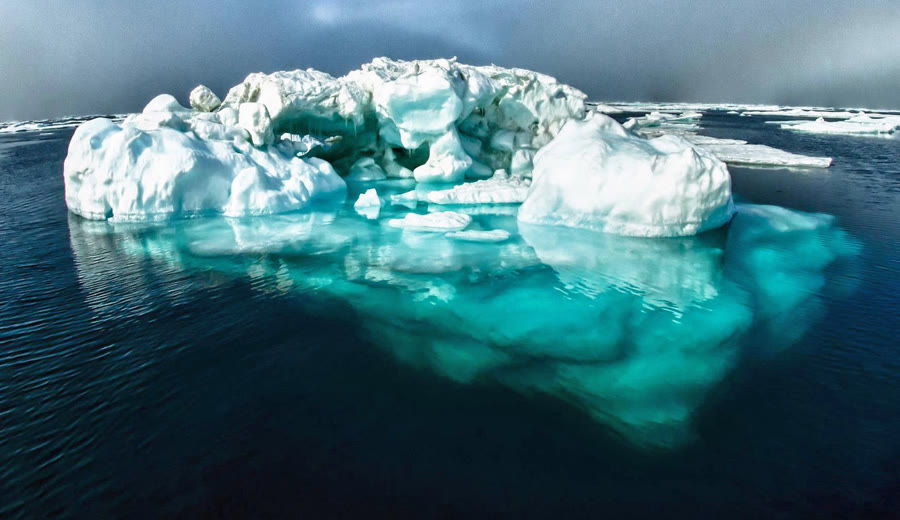
\includegraphics[width=0.66\linewidth]{images/book2/g11-noaa-iceberg.jpg}

{\small जल के ठीक ऊपर से दिखता एक हिमशैल: सतह के नीचे की बर्फ़,
जो स्वच्छ समुद्र में से झलकती है, हवा में के भाग से कहीं बड़ी है।
फ़ोटो: NOAA (सार्वजनिक डोमेन)।}
\end{omfigure}
% ledger: photo:g11-iceberg

\section{पृथ्वी को परतों में बाँटने के दो ढंग}

भूपर्पटी, प्रावार और क्रोड अलग-अलग
\emph{पदार्थों} की परतें हैं: भूपर्पटी सिलिकॉन, ऐलुमिनियम और
ऑक्सीजन से समृद्ध चट्टानों से बनी है, प्रावार एक अधिक घनी चट्टान से, क्रोड धातु से। पर
पृथ्वी के बाहरी भाग को इस आधार पर भी बाँटा जा सकता है कि उसकी चट्टान बहुत लंबे समय तक
उस पर बल लगने पर कैसा \emph{व्यवहार} करती है।

\begin{definition}[स्थलमंडल; दुर्बलतामंडल]\label{def:g11:lithosphere-asthenosphere:lithosphere}
\emph{स्थलमंडल}\index{स्थलमंडल} पृथ्वी का कठोर बाहरी
कवच है: भूपर्पटी और प्रावार का सबसे ऊपरी, सबसे ठंडा भाग, जो मिलकर
विवर्तनिक प्लेटों में टूटते हैं और बहते नहीं। \emph{दुर्बलतामंडल}\index{दुर्बलतामंडल}
स्थलमंडल के नीचे की प्रावार की परत है, अधिक गरम और अधिक दुर्बल, जो लंबी
अवधियों में धीरे-धीरे बहती है, किसी बहुत कड़े लेप की तरह।
\end{definition}

दोनों के बीच की सीमा महासागरों और अधिकांश महाद्वीपों के नीचे लगभग 70 से \qty{100}{km} नीचे है,
और महाद्वीपों के सबसे पुराने भागों के नीचे अधिक गहरी; उदाहरण के लिए, संयुक्त राज्य अमेरिका के आर-पार
\omterm{def:g11:lithosphere-asthenosphere:lithosphere}{स्थलमंडल} पश्चिम में लगभग \qty{40}{km} मोटा है और महाद्वीप के मध्य में
\qty{200}{km} से अधिक मोटा। \omterm{def:g11:lithosphere-asthenosphere:lithosphere}{स्थलमंडल} का आधार \omterm{def:g11:seismic-structure:moho}{मोहो} नहीं है:
\omterm{def:g11:lithosphere-asthenosphere:lithosphere}{स्थलमंडल} का अधिकांश भाग प्रावार की चट्टान है।
% ledger: rs09:lab, fischer:lab, porter:lab, usgs:lithosphere-80km (Book 1 row)

\begin{omfigure}
\begin{tikzpicture}[x=1cm, y=-0.0125cm, font=\footnotesize]
% depths to scale: crust 41 km (cm95:crust), lithosphere 100 km (rs09:lab), 0-400 km
  \shade[top color=omLithPeridotite!70, bottom color=omLithPeridotite!25] (5,100) rectangle (8,400);
  \fill[omLithGranite!55] (0,0) rectangle (3,41);
  \fill[omLithPeridotite!55] (0,41) rectangle (3,400);
  \fill[black!25] (5,0) rectangle (8,100);
  \draw (0,0) rectangle (3,400);
  \draw (5,0) -- (5,400) (8,0) -- (8,400) (5,0) -- (8,0);
  \draw[line width=0.8pt] (0,41) -- (3,41);
  \draw[line width=0.8pt, densely dashed] (5,100) -- (8,100);
  \draw[densely dotted, black!60] (3,41) -- (5,41);
  \node at (1.5,20) {भूपर्पटी};
  \node[align=center] at (1.5,220) {प्रावार};
  \node[align=center] at (6.5,50) {स्थलमंडल\\कठोर};
  \node[align=center] at (6.5,180) {दुर्बलतामंडल\\दुर्बल, धीरे बहता है};
  \node[align=center, text=black!70] at (6.5,340) {अधिक गहरा प्रावार};
  \node[anchor=south, font=\small] at (1.5,0) {पदार्थ के अनुसार};
  \node[anchor=south, font=\small] at (6.5,0) {व्यवहार के अनुसार};
  \foreach \d in {0,100,200,300,400} {\draw (-0.1,\d) -- (0,\d); \node[anchor=east] at (-0.1,\d) {\d};}
  \node[anchor=east, rotate=90, anchor=south] at (-0.9,200) {गहराई (\unit{km})};
  \node[anchor=south, font=\scriptsize, align=center] at (4,41) {मोहो\\(\qty{41}{km})};
  \node[anchor=west, align=left] at (8.15,100) {स्थलमंडल\\का आधार\\(लगभग \qty{100}{km})};
\end{tikzpicture}

{\small किसी महाद्वीप के नीचे पृथ्वी के ऊपरी \qty{400}{km}, पैमाने पर।
बाएँ: पदार्थ के अनुसार परतें। दाएँ: व्यवहार के अनुसार परतें। कठोर
\omterm{def:g11:lithosphere-asthenosphere:lithosphere}{स्थलमंडल} में पूरी भूपर्पटी और प्रावार का ऊपरी भाग आता है;
\omterm{def:g11:lithosphere-asthenosphere:lithosphere}{दुर्बलतामंडल} की कोई स्पष्ट निचली सीमा नहीं है।}
\end{omfigure}

\section{निम्न-वेग क्षेत्र}

भूकंपीय तरंगें \omterm{def:g11:lithosphere-asthenosphere:lithosphere}{दुर्बलतामंडल} को दिखाती हैं। पृथ्वी में लगभग हर जगह भूकंपीय
चालें गहराई के साथ बढ़ती हैं, क्योंकि चट्टान अधिकाधिक दबती जाती है।
\omterm{def:g11:lithosphere-asthenosphere:lithosphere}{स्थलमंडल} के नीचे इसका उलटा होता है।

\begin{definition}[निम्न-वेग क्षेत्र]\label{def:g11:lithosphere-asthenosphere:lvz}
\emph{निम्न-वेग क्षेत्र}\index{निम्न-वेग क्षेत्र} \omterm{def:g11:lithosphere-asthenosphere:lithosphere}{स्थलमंडल} के नीचे ऊपरी
प्रावार की वह परत है जिसमें भूकंपीय तरंगें अपने ऊपर और नीचे की चट्टान की अपेक्षा
अधिक धीरे चलती हैं।
\end{definition}

\omterm{def:g11:seismic-structure:reference-model}{संदर्भ पृथ्वी मॉडल} में S चाल \omterm{def:g11:seismic-structure:moho}{मोहो} से
\qty{220}{km} तक धीरे-धीरे घटती है, फिर उछलकर बढ़ती है। पूरे संसार के भूकंपीय अध्ययन
70 और \qty{100}{km} के बीच कहीं चाल में एक तीव्र गिरावट पाते हैं: यह
\omterm{def:g11:lithosphere-asthenosphere:lithosphere}{दुर्बलतामंडल} का शीर्ष है। वहाँ की चट्टान पिघलने के निकट होने लायक गरम है, और उसमें
बहुत थोड़ा पिघला पदार्थ हो सकता है; उसमें ऊपर की चट्टान से अधिक जल भी हो सकता है।
पिघलने के निकट की चट्टान दुर्बल होती है: वह भूकंपीय तरंगों को धीमा करती है, और बह सकती है।
% ledger: data:prem, rs09:lab, fischer:lab, porter:lab

\begin{omfigure}
\begin{tikzpicture}
\begin{axis}[omrecord, omdepth, width=0.6\linewidth, height=6.0cm, xmin=3.0, xmax=5.0, ymin=0, ymax=400,
  xlabel={S चाल (\unit{km/s})}, ylabel={गहराई (\unit{km})}, xtick={3.0,3.5,...,5.0},
  xticklabel style={/pgf/number format/fixed, /pgf/number format/precision=1},
  tick label style={font=\small}, label style={font=\small}]
% computed in figdata/grade-11/prem_profiles.py (part upper); ledger: data:prem
\fill[black!10] (axis cs:3.0,80) rectangle (axis cs:5.0,220);
\addplot[omProp, line width=0.9pt] table[x=vs, y=depth] {figdata/out/grade-11-prem_profiles-upper.dat};
\node[font=\scriptsize, anchor=west, align=left] at (axis cs:3.1,150) {निम्न-वेग\\क्षेत्र};
\node[font=\scriptsize, anchor=west] at (axis cs:3.95,12) {भूपर्पटी};
\end{axis}
\end{tikzpicture}

{\small \omterm{def:g11:seismic-structure:reference-model}{संदर्भ पृथ्वी मॉडल} के ऊपरी \qty{400}{km} में S चाल।
भूपर्पटी के नीचे चाल गहराई के साथ
\qty{220}{km} तक धीरे-धीरे घटती है (\qty{80}{km} से छायांकित), फिर एकाएक
उछालों के साथ फिर बढ़ती है।}
\end{omfigure}

\section{भूतापीय वक्र}

\begin{definition}[भूतापीय वक्र; भूतापीय प्रवणता]\label{def:g11:lithosphere-asthenosphere:geotherm}
\emph{भूतापीय वक्र}\index{भूतापीय वक्र} किसी स्थान के नीचे गहराई के सापेक्ष
तापमान का वक्र है। \emph{भूतापीय प्रवणता}\index{भूतापीय प्रवणता}
गहराई की प्रति इकाई तापमान की वृद्धि है, अंश प्रति किलोमीटर में।
\end{definition}

वेधछिद्र \omterm{def:g11:lithosphere-asthenosphere:geotherm}{भूतापीय वक्र} को केवल पहले कुछ किलोमीटर में मापते हैं, जहाँ
तापमान 25 से \qty{30}{\celsius} प्रति किलोमीटर बढ़ता है (पुस्तक 1,
कक्षा 6)। अधिक गहराई पर इसे सतह से बाहर बहने वाली ऊष्मा से
और चट्टानों के गुणों से परिकलित किया जाता है; \cref{ch:g12:internal-heat}
दिखाता है कि वह ऊष्मा कहाँ से आती है। दो तथ्य परिणाम को आकार देते हैं। ऊष्मा का
एक भाग स्वयं ऊपरी भूपर्पटी के भीतर बनता है, इसलिए प्रवणता सतह के पास
सबसे तीव्र और भूपर्पटी के नीचे कम होती है। और \omterm{def:g11:lithosphere-asthenosphere:lithosphere}{दुर्बलतामंडल} में, जो
बहता है, चट्टान की धीमी गति ऊष्मा ले जाती है और तापमान को
समान कर देती है: वह प्रति किलोमीटर केवल लगभग \qty{0.45}{\celsius} बढ़ता है।
\omterm{def:g11:lithosphere-asthenosphere:lithosphere}{स्थलमंडल} का आधार वहाँ माना जाता है जहाँ \omterm{def:g11:lithosphere-asthenosphere:lithosphere}{स्थलमंडल} का तीव्र \omterm{def:g11:lithosphere-asthenosphere:geotherm}{भूतापीय वक्र}
\omterm{def:g11:lithosphere-asthenosphere:lithosphere}{दुर्बलतामंडल} के मंद वक्र से मिलता है, लगभग \qty{1300}{\celsius} पर।
% ledger: usgs:gradient-29 (Book 1 row), b2dd10:continents, b2roy:provinces, roy:conductivity,
% katsura10:adiabat, porter:lab

\begin{omfigure}
\begin{tikzpicture}
\begin{axis}[omrecord, omdepth, width=0.7\linewidth, height=6.4cm, xmin=0, xmax=2000, ymin=0, ymax=300,
  xlabel={तापमान (\unit{\celsius})}, ylabel={गहराई (\unit{km})}, xtick={0,500,...,2000},
  tick label style={font=\small}, label style={font=\small}]
% computed in figdata/grade-11/geotherm_solidus.py; ledger: b2dd10:continents, b2roy:provinces,
% roy:conductivity, porter:lab, katsura10:adiabat, hirschmann:solidus, data:prem
\fill[black!8] (axis cs:0,99.7) rectangle (axis cs:2000,300);
\addplot[omDef, line width=1.0pt] table[x=t_geotherm, y=depth_km] {figdata/out/grade-11-geotherm_solidus-geotherm.dat};
\addplot[omDef, densely dashed, restrict y to domain=99:300] table[x=t_cond, y=depth_km] {figdata/out/grade-11-geotherm_solidus-geotherm.dat};
\addplot[omProp, line width=1.0pt] table[x=t_solidus, y=depth_km] {figdata/out/grade-11-geotherm_solidus-geotherm.dat};
\draw[black!60] (axis cs:0,99.7) -- (axis cs:2000,99.7);
\node[font=\scriptsize, anchor=south west] at (axis cs:20,99.7) {स्थलमंडल का आधार};
\node[font=\scriptsize, anchor=north west] at (axis cs:20,102) {दुर्बलतामंडल};
\node[font=\scriptsize, text=omDef, anchor=north west] at (axis cs:480,6) {भूतापीय वक्र};
\node[font=\scriptsize, text=omProp, anchor=west] at (axis cs:1300,22) {पिघलना शुरू};
\end{axis}
\end{tikzpicture}

{\small किसी महाद्वीप के नीचे एक मॉडल \omterm{def:g11:lithosphere-asthenosphere:geotherm}{भूतापीय वक्र} (नीला) और वह तापमान जिस पर
प्रावार की चट्टान (पेरिडोटाइट, बिना जल के) पिघलना शुरू करती है (नारंगी)।
\omterm{def:g11:lithosphere-asthenosphere:geotherm}{भूतापीय वक्र} महाद्वीपों के माध्य ऊष्मा-प्रवाह और चट्टानों के मापे गए
गुणों से परिकलित है; \omterm{def:g11:lithosphere-asthenosphere:lithosphere}{दुर्बलतामंडल} (धूसर) में वह धीरे-धीरे बढ़ता है। डैश रेखा दिखाती है
कि \omterm{def:g11:lithosphere-asthenosphere:lithosphere}{स्थलमंडल} की अधिक तीव्र वृद्धि कैसे जारी रहती। दोनों वक्र
\omterm{def:g11:lithosphere-asthenosphere:lithosphere}{स्थलमंडल} के आधार के पास सबसे निकट आते हैं, लगभग \qty{140}{\celsius} के अंतर पर।}
\end{omfigure}
% values: lab_km 99.7, t_lab_c 1345, closest_gap_c 144 (figdata/grade-11/geotherm_solidus.py)

प्रावार की चट्टान का गलनांक गहराई के साथ बढ़ता है, क्योंकि
चट्टान अधिकाधिक दबती जाती है (पुस्तक 1, कक्षा 6): सतह पर लगभग \qty{1120}{\celsius},
\qty{100}{km} पर लगभग \qty{1500}{\celsius}। मॉडल में
\omterm{def:g11:lithosphere-asthenosphere:geotherm}{भूतापीय वक्र} \omterm{def:g11:lithosphere-asthenosphere:lithosphere}{स्थलमंडल} के ठीक नीचे उसके सबसे निकट आता है, उससे लगभग
\qty{140}{\celsius} कम। थोड़ा-सा जल, या थोड़ा अधिक गरम
प्रावार, यह अंतर पाट देता है: संयुक्त राज्य अमेरिका के पश्चिम में, जहाँ
\omterm{def:g11:lithosphere-asthenosphere:lithosphere}{स्थलमंडल} पतला है, उसके नीचे के प्रावार का थोड़ा भाग आंशिक रूप से पिघला है।
% ledger: hirschmann:solidus, porter:lab; computed in figdata/grade-11/geotherm_solidus.py
% (solidus0_c 1120.7, solidus100_c 1489, closest_gap_c 144)

\section{समस्थिति}

\subsection{किसी ठोस पर तैरना}

भूकंप की तरंग के कुछ सेकंडों में \omterm{def:g11:lithosphere-asthenosphere:lithosphere}{दुर्बलतामंडल} ठोस है। लंबी
अवधियों में वह बहता है। \omterm{def:g11:lithosphere-asthenosphere:lithosphere}{स्थलमंडल} पर रखा गया भार --- कोई पर्वत-श्रेणी,
कोई हिमचादर --- \omterm{def:g11:lithosphere-asthenosphere:lithosphere}{दुर्बलतामंडल} को धीरे-धीरे तब तक हटाता है जब तक भार
तैरने न लगे, जैसे जल पर लकड़ी का एक गुटका।

\begin{definition}[समस्थिति; क्षतिपूर्ति गहराई]\label{def:g11:lithosphere-asthenosphere:isostasy}
\emph{समस्थिति}\index{समस्थिति} वह संतुलन है जिसमें पृथ्वी की बाहरी
परतें \omterm{def:g11:lithosphere-asthenosphere:lithosphere}{दुर्बलतामंडल} पर तैरती हैं: प्रावार में एक गहराई पर, जिसे
\emph{क्षतिपूर्ति गहराई}\index{क्षतिपूर्ति गहराई} कहते हैं, सतह से उस गहराई तक
समान अनुप्रस्थ काट वाले चट्टान के हर स्तंभ का भार समान होता है,
उसके ऊपर का उच्चावच चाहे जैसा हो।
\end{definition}

\begin{omfigure}
\begin{tikzpicture}[x=1cm, y=1cm, font=\footnotesize, >={Stealth[length=4pt]}]
% not to scale
  \fill[omSea!50] (6,0) rectangle (8.6,-0.9);
  \fill[omLithPeridotite!45] (0,-5.2) rectangle (2.6,-6.6);
  \fill[omLithGranite!55] (0,2.0) -- (2.6,2.0) -- (2.6,-5.2) -- (0,-5.2) -- cycle;
  \fill[omLithGranite!55] (2.6,0) rectangle (6,-3.0);
  \fill[omLithGranite!55] (6,-0.9) rectangle (8.6,-1.6); % same fill: one crustal density in Airy's model
  \fill[omLithPeridotite!45] (2.6,-3.0) rectangle (6,-6.6);
  \fill[omLithPeridotite!45] (6,-1.6) rectangle (8.6,-6.6);
  \draw (0,2.0) -- (2.6,2.0) -- (2.6,0) -- (6,0);
  \draw (6,0) -- (8.6,0);
  \draw[line width=0.8pt] (0,-5.2) -- (2.6,-5.2) -- (2.6,-3.0) -- (6,-3.0) -- (6,-1.6) -- (8.6,-1.6);
  \draw[densely dashed, line width=0.8pt] (0,-6.2) -- (8.6,-6.2);
  \node[anchor=north east] at (8.6,-6.6) {क्षतिपूर्ति गहराई};
  \draw[black!50, densely dotted] (-0.2,0) -- (0,0);
  \node[anchor=east] at (-0.2,0) {समुद्र-तल};
  \node at (1.3,-1.6) {भूपर्पटी};
  \node at (4.3,-1.5) {भूपर्पटी};
  \node at (7.3,-0.45) {महासागर};
  \node at (7.3,-1.25) {भूपर्पटी};
  \node at (4.3,-4.8) {प्रावार};
  \node[anchor=south] at (1.3,2.0) {पर्वत-श्रेणी};
  \node[anchor=south] at (4.3,0) {निचली भूमि};
  \draw[<->] (2.75,0) -- (2.75,2.0); \node[anchor=west] at (2.8,1.0) {$h$};
  \draw[<->] (2.75,-3.0) -- (2.75,-5.2); \node[anchor=west] at (2.8,-4.1) {मूल $r$};
  \draw[<->] (5.85,0) -- (5.85,-3.0); \node[anchor=east] at (5.8,-1.0) {$T$};
\end{tikzpicture}

{\small \omterm{def:g11:lithosphere-asthenosphere:isostasy}{समस्थिति} का एयरी मॉडल (पैमाने पर नहीं)। भूपर्पटी का घनत्व हर जगह
एक-सा है; जहाँ वह ऊँची उठी है, वहाँ वह मोटी है और उसका एक मूल है जो
अधिक घने प्रावार में गहराई तक जाता है। महासागर के नीचे भूपर्पटी पतली है। तीनों
स्तंभों का भार \omterm{def:g11:lithosphere-asthenosphere:isostasy}{क्षतिपूर्ति गहराई} तक समान है।}
\end{omfigure}

\subsection{पर्वत-श्रेणी का मूल}

\begin{proposition}[एयरी समस्थिति]\label{prop:g11:lithosphere-asthenosphere:airy}
मान लीजिए भूपर्पटी का एकसमान घनत्व $\rho_c$ है, और उसके नीचे के प्रावार का
घनत्व $\rho_m > \rho_c$। यदि कोई क्षेत्र किसी दूसरे क्षेत्र से ऊँचाई $h$ ऊपर है
और दोनों समस्थितिक संतुलन में हैं, तो उसकी भूपर्पटी इतनी अधिक मोटी है:
\[
  \Delta H = h\,\frac{\rho_m}{\rho_m - \rho_c},
\]
जिसमें से $h$ दूसरे क्षेत्र से ऊपर है और एक मूल
$r = h\,\rho_c/(\rho_m - \rho_c)$ उसकी भूपर्पटी के नीचे पहुँचता है।\index{एयरी समस्थिति}
\end{proposition}

\begin{proof}
समान क्षेत्रफल $S$ के दो स्तंभ लीजिए: निचली भूमि का, जिसकी भूपर्पटी की मोटाई
$T$ है, और श्रेणी का, जिसकी भूपर्पटी $h$ अधिक ऊँची है और $r$ अधिक गहराई तक जाती है, जिससे
उसकी मोटाई $T + h + r$ है। दोनों \omterm{def:g11:seismic-structure:moho}{मोहो} के नीचे की किसी \omterm{def:g11:lithosphere-asthenosphere:isostasy}{क्षतिपूर्ति गहराई} तक,
श्रेणी के स्तंभ में $h + r$ अधिक भूपर्पटी है; निचली भूमि के स्तंभ में
उसके बजाय मोटाई $r$ तक प्रावार है। $g$ को गुरुत्वीय त्वरण मानकर,
दोनों भार तब बराबर हैं जब
\[
  \rho_c\,(h + r)\,S\,g = \rho_m\,r\,S\,g,
  \qquad\text{यानी}\qquad
  r = h\,\frac{\rho_c}{\rho_m - \rho_c}.
\]
भूपर्पटी $h + r = h\,\bigl(1 + \rho_c/(\rho_m - \rho_c)\bigr)
= h\,\rho_m/(\rho_m - \rho_c)$ अधिक मोटी है।
\end{proof}

यदि महाद्वीपीय भूपर्पटी का माध्य घनत्व $\rho_c =
\qty{2830}{kg/m^3}$ लें, और \omterm{def:g11:seismic-structure:moho}{मोहो} के ठीक नीचे के प्रावार का घनत्व $\rho_m =
\qty{3380}{kg/m^3}$, तो मूल ऊँचाई का $2830/550 \approx 5.1$ गुना है,
और भूपर्पटी ऊँचाई के लगभग $6.1$ गुना अधिक मोटी है: अपने परिवेश से
\qty{3}{km} ऊँची श्रेणी का मूल लगभग \qty{15}{km} होता है।
% ledger: cm95:crust, data:prem (rho 3.38 below the Moho)

\begin{method}[मूल का परिकलन]\label{met:g11:lithosphere-asthenosphere:root}
\begin{enumerate}
  \item ऐसे संदर्भ क्षेत्र से, जिसकी भूपर्पटी की मोटाई ज्ञात हो, क्षेत्र की ऊँचाई $h$
        ज्ञात कीजिए।
  \item भूपर्पटी और प्रावार के घनत्वों से $\rho_m/(\rho_m - \rho_c)$
        परिकलित कीजिए।
  \item भूपर्पटी संदर्भ भूपर्पटी से $h\,\rho_m/(\rho_m -
        \rho_c)$ अधिक मोटी है; अकेला मूल उसमें से $h$ घटाने पर मिलता है।
\end{enumerate}
\end{method}

\begin{example}[\qty{2}{km} ऊँचा एक पठार]\label{ex:g11:lithosphere-asthenosphere:plateau}
एक पठार ऐसी निचली भूमि से \qty{2}{km} ऊपर है जिसकी भूपर्पटी \qty{37}{km}
मोटी है। उसकी भूपर्पटी $2 \times 3380/550 \approx \qty{12.3}{km}$ अधिक मोटी है:
कुल लगभग \qty{49}{km}, लगभग \qty{10}{km} के मूल के साथ।
\end{example}

\subsection{महाद्वीप ऊँचे क्यों हैं}

\begin{definition}[उच्चतामितीय वक्र]\label{def:g11:lithosphere-asthenosphere:hypsometry}
पृथ्वी का \emph{उच्चतामितीय वक्र}\index{उच्चतामितीय वक्र} हर
ऊँचाई के लिए पृथ्वी की सतह का वह भिन्न देता है जो उससे ऊँचा है।
उसकी ढाल दिखाती है कि सतह का कितना भाग हर ऊँचाई पर है।
\end{definition}

यदि सतह संयोग से आकार लेती, तो उसका अधिकांश भाग किसी एक
औसत तल के पास होता। ऐसा नहीं है।

\begin{proposition}[दो तल]\label{prop:g11:lithosphere-asthenosphere:two-levels}
पृथ्वी की सतह की ऊँचाइयाँ दो तलों के आसपास जमा हैं: एक समुद्र-तल से
कुछ सौ मीटर के भीतर, महाद्वीपों पर, और एक समुद्र-तल से लगभग 4 से
\qty{5}{km} नीचे, गहरी महासागरीय तली पर। स्थल सतह का \qty{29}{\percent}
ढकता है; सतह का आधे से अधिक भाग समुद्र-तल से \qty{3}{km} से अधिक
नीचे है, और केवल \qty{3}{\percent} भाग \qty{2}{km} से अधिक ऊँचा उठता है।
\end{proposition}
% computed in figdata/grade-11/hypsometry.py from ETOPO1 (land_fraction 0.290,
% share_below_3000_pct 53.4, share_above_2000_pct 3.1; modes at +250 and -4250 m); ledger: data:etopo1

\begin{omfigure}
\begin{tikzpicture}
\begin{axis}[omrecord, width=0.86\linewidth, height=5.4cm, xmin=-11000, xmax=9000, ymin=0, ymax=18,
  xlabel={ऊँचाई (\unit{m}; ऋणात्मक: समुद्र-तल से नीचे)}, ylabel={सतह का अंश (\unit{\percent})},
  xtick={-10000,-8000,...,8000}, scaled x ticks=false, xticklabel style={/pgf/number format/1000 sep={\,}, font=\scriptsize},
  tick label style={font=\small}, label style={font=\small}, clip=false]
% computed in figdata/grade-11/hypsometry.py; ledger: data:etopo1
\addplot[ybar interval, fill=omSea!70, draw=black!50, restrict expr to domain={\thisrow{land}}{0:0}] table[x=lo, y=share_pct] {figdata/out/grade-11-hypsometry-bins.dat};
\addplot[ybar interval, fill=omHypsLandC, draw=black!50, restrict expr to domain={\thisrow{land}}{1:1}] table[x=lo, y=share_pct] {figdata/out/grade-11-hypsometry-bins.dat};
\draw[black!60, densely dotted] (axis cs:0,0) -- (axis cs:0,18);
\node[font=\scriptsize, anchor=south west] at (axis cs:600,15.5) {महाद्वीप};
\node[font=\scriptsize, anchor=south] at (axis cs:-4250,12.2) {गहरी महासागरीय तली};
\end{axis}
\end{tikzpicture}

{\small ऊँचाई की \qty{500}{m} की हर पट्टी में पृथ्वी की सतह का अंश
(ETOPO1 से, एक अंश के विभेदन पर; अंटार्कटिका और ग्रीनलैंड पर
बर्फ़ का शीर्ष)। दोनों शिखर महाद्वीप और गहरी महासागरीय तली हैं।}
\end{omfigure}

\omterm{def:g11:lithosphere-asthenosphere:isostasy}{समस्थिति} दोनों तलों को समझाती है। महाद्वीप हल्की चट्टान की मोटी भूपर्पटी से बने हैं,
औसतन लगभग \qty{41}{km}; महासागरीय तली अधिक घनी चट्टान की पतली भूपर्पटी से,
केवल लगभग \qty{5}{km} मोटी। दोनों
\omterm{def:g11:lithosphere-asthenosphere:lithosphere}{दुर्बलतामंडल} पर तैरती हैं: मोटी, हल्की महाद्वीपीय भूपर्पटी ऊँचे तैरती है, पतली, घनी
महासागरीय भूपर्पटी नीचे, और महासागर निचली भूमि को भर देते हैं।
% ledger: cm95:crust, usgs:crust-thickness (Book 1 row)

\section{एक लचीला ढक्कन}

\omterm{def:g11:lithosphere-asthenosphere:isostasy}{समस्थिति} के लिए आवश्यक है कि \omterm{def:g11:lithosphere-asthenosphere:lithosphere}{दुर्बलतामंडल} बहे। उसके ऊपर का \omterm{def:g11:lithosphere-asthenosphere:lithosphere}{स्थलमंडल} नहीं
बहता; वह झुकता है। \omterm{def:g11:lithosphere-asthenosphere:lithosphere}{स्थलमंडल} की मोटाई से संकरा भार, जैसे
एक अकेला ज्वालामुखीय द्वीप, प्लेट की कठोरता से सँभाला जाता है, जैसे
किसी तख़्ते पर रखा भार, और प्लेट उसके चारों ओर नीचे झुक जाती है। उस मोटाई से
बहुत चौड़ा भार, जैसे पूरी पर्वत-श्रेणी या कोई हिमचादर, तब तक धँसता है जब तक
तैरने न लगे। भार हट जाने पर \omterm{def:g11:lithosphere-asthenosphere:lithosphere}{स्थलमंडल} धीरे-धीरे फिर ऊपर उठता है
(\cref{ch:g12:destruction-of-mountains})।

\section{अभ्यास}

\begin{exercise}[$\star$]\label{exo:g11:lithosphere-asthenosphere:1}
\omterm{def:g11:lithosphere-asthenosphere:lithosphere}{स्थलमंडल} और \omterm{def:g11:lithosphere-asthenosphere:lithosphere}{दुर्बलतामंडल} की परिभाषा दीजिए। निम्नलिखित में से कौन-से
\omterm{def:g11:lithosphere-asthenosphere:lithosphere}{स्थलमंडल} के अंग हैं: महासागरीय भूपर्पटी, महाद्वीपीय भूपर्पटी, सबसे ऊपरी
प्रावार, बाह्य क्रोड?
\end{exercise}

\begin{exercise}[$\star$]\label{exo:g11:lithosphere-asthenosphere:2}
\qty{910}{kg/m^3} घनत्व का एक हिमशैल \qty{1025}{kg/m^3} घनत्व वाले समुद्री जल में
तैरता है। उसके आयतन का कितना भाग जल के नीचे है? यदि
ऊर्ध्वाधर किनारों वाला एक हिमशैल जल से \qty{20}{m} ऊपर उठा है, तो उसकी
कुल ऊँचाई क्या है?
\end{exercise}

\begin{exercise}[$\star$]\label{exo:g11:lithosphere-asthenosphere:3}
ज़मीन \qty{15}{\celsius} पर है और \omterm{def:g11:lithosphere-asthenosphere:geotherm}{भूतापीय प्रवणता}
\qty{26}{\celsius} प्रति किलोमीटर है। \qty{3}{km} गहरे वेधछिद्र के तल पर
तापमान क्या है? वही प्रवणता \qty{100}{km} तक क्यों
नहीं प्रयुक्त की जा सकती?
\end{exercise}

\begin{exercise}[$\star$]\label{exo:g11:lithosphere-asthenosphere:4}
पृथ्वी की सतह की ऊँचाइयों वाले चित्र से ऊँचाई की दो सबसे
सामान्य पट्टियाँ और हर एक में सतह का अंश बताइए।
\end{exercise}

\begin{exercise}[$\star$]\label{exo:g11:lithosphere-asthenosphere:5}
सूत्र $T = -5.104\,P^2 + 132.899\,P + 1120.661$ (तापमान
\unit{\celsius} में, दाब $P$ गीगापास्कल में) से वह तापमान परिकलित कीजिए
जिस पर शुष्क प्रावार-चट्टान सतह पर ($P = 0$) और
\qty{3}{GPa} पर, लगभग \qty{95}{km} नीचे, पिघलना शुरू करती है।
\end{exercise}

\begin{exercise}[$\star\star$]\label{exo:g11:lithosphere-asthenosphere:6}
मॉडल \omterm{def:g11:lithosphere-asthenosphere:geotherm}{भूतापीय वक्र} के चित्र पर 50, 150 और
\qty{250}{km} पर तापमान पढ़िए। हर गहराई किस परत में है, \omterm{def:g11:lithosphere-asthenosphere:lithosphere}{स्थलमंडल} या \omterm{def:g11:lithosphere-asthenosphere:lithosphere}{दुर्बलतामंडल}?
इनमें से किन दो गहराइयों के बीच तापमान सबसे अधिक बढ़ता है?
\end{exercise}

\begin{exercise}[$\star\star$]\label{exo:g11:lithosphere-asthenosphere:7}
एक पर्वत-श्रेणी किसी निचली भूमि से \qty{3}{km} ऊपर है; $\rho_c =
\qty{2830}{kg/m^3}$ और $\rho_m = \qty{3380}{kg/m^3}$ लीजिए। उसका मूल और
उसकी भूपर्पटी की अतिरिक्त मोटाई परिकलित कीजिए।
\end{exercise}

\begin{exercise}[$\star\star$]\label{exo:g11:lithosphere-asthenosphere:8}
किसी क्षेत्र की भूपर्पटी \qty{55}{km} मोटी है।
\cref{exo:g11:lithosphere-asthenosphere:7} के घनत्वों के साथ, वह ऐसे
क्षेत्र से कितना ऊँचा है जिसकी भूपर्पटी \qty{41.1}{km} मोटी है?
\end{exercise}

\begin{exercise}[$\star\star$]\label{exo:g11:lithosphere-asthenosphere:9}
संदर्भ मॉडल में S चाल \qty{80}{km} पर \qty{4.470}{km/s},
\qty{220}{km} के ठीक ऊपर \qty{4.419}{km/s} और ठीक नीचे \qty{4.644}{km/s} है।
80 और \qty{220}{km} के बीच की कमी और \qty{220}{km} पर के उछाल को
प्रतिशत में परिकलित कीजिए। गहराई के साथ चाल का घटना आश्चर्यजनक क्यों है?
\end{exercise}

\begin{exercise}[$\star\star$]\label{exo:g11:lithosphere-asthenosphere:10}
मॉडल \omterm{def:g11:lithosphere-asthenosphere:geotherm}{भूतापीय वक्र} में तापमान \qty{40}{km} नीचे \omterm{def:g11:seismic-structure:moho}{मोहो} पर \qty{610}{\celsius}
और \qty{100}{km} नीचे \omterm{def:g11:lithosphere-asthenosphere:lithosphere}{स्थलमंडल} के आधार पर \qty{1345}{\celsius} है।
(1) दोनों के बीच की माध्य प्रवणता परिकलित कीजिए। (2)
सतह की प्रवणता, \qty{26}{\celsius} प्रति किलोमीटर, से तुलना कीजिए,
और अंतर समझाइए।
\end{exercise}

\begin{exercise}[$\star\star$]\label{exo:g11:lithosphere-asthenosphere:11}
\omterm{def:g11:lithosphere-asthenosphere:lithosphere}{दुर्बलतामंडल} में तापमान $1300 + 0.45\,z$ लिया जाता है
(\unit{\celsius} में, $z$ किलोमीटर में)। इसे 200 और \qty{400}{km} पर परिकलित कीजिए। दोनों के
बीच यह कितना बढ़ता है? इसकी तुलना पहले \qty{100}{km} में हुई वृद्धि से कीजिए,
सतह पर \qty{15}{\celsius} से \omterm{def:g11:lithosphere-asthenosphere:lithosphere}{स्थलमंडल} के आधार पर
\qty{1345}{\celsius} तक।
\end{exercise}

\begin{exercise}[$\star\star\star$]\label{exo:g11:lithosphere-asthenosphere:12}
ऊपरी भूपर्पटी के नीचे मॉडल \omterm{def:g11:lithosphere-asthenosphere:geotherm}{भूतापीय वक्र} लगभग $T \approx 118 +
G\,z$ है (\unit{\celsius} में, $z$ किलोमीटर में), जहाँ प्रवणता $G$
अधिक गहराई से आने वाली ऊष्मा पर निर्भर करती है। (1) $G =
\qty{12.3}{\celsius}$ प्रति किलोमीटर के लिए, जैसा संयुक्त राज्य अमेरिका के पूर्व के लिए
परिकलित है, वह गहराई ज्ञात कीजिए जिस पर यह $1300 + 0.45\,z$ से मिलता है। (2) यही
$G = \qty{21.5}{\celsius}$ प्रति किलोमीटर के लिए कीजिए, जैसा पश्चिम के द्रोणी-और-श्रेणी
प्रांत के लिए परिकलित है। (3) मापी गई मोटाइयों से तुलना कीजिए, जो पश्चिम में लगभग
\qty{40}{km} से लेकर महाद्वीप के मध्य में \qty{200}{km} से अधिक तक हैं।
\end{exercise}

\begin{exercise}[$\star\star\star$]\label{exo:g11:lithosphere-asthenosphere:13}
(1) दिखाइए कि एयरी के मॉडल में, जिस क्षेत्र की भूपर्पटी किसी संदर्भ क्षेत्र से $\Delta H$ अधिक
मोटी है, वह $\Delta H\,(\rho_m - \rho_c)/\rho_m$ अधिक ऊँचा है।
(2) भूपर्पटी की किसी भी अतिरिक्त मोटाई का कितना भाग ऊँचाई के रूप में दिखता है? (3)
हिमशैल के जल से ऊपर के भाग से तुलना कीजिए।
\end{exercise}

\begin{exercise}[$\star\star\star$]\label{exo:g11:lithosphere-asthenosphere:14}
\qty{100}{km} पर शुष्क प्रावार-चट्टान \qty{1489}{\celsius} पर पिघलना शुरू करती है,
और मॉडल \omterm{def:g11:lithosphere-asthenosphere:geotherm}{भूतापीय वक्र} \qty{1345}{\celsius} पर है। (1) वहाँ चट्टान के पिघलना शुरू करने के लिए
जल को गलनांक कितने अंश घटाना होगा? (2) पिघले पदार्थ का बहुत छोटा अंश भी
चट्टान को दुर्बल क्यों कर देगा और भूकंपीय तरंगों को धीमा क्यों कर देगा?
\end{exercise}

\begin{exercise}[$\star\star\star$]\label{exo:g11:lithosphere-asthenosphere:15}
पृथ्वी की सतह का केवल \qty{3}{\percent} भाग \qty{2}{km} से ऊपर उठता है, जबकि
\qty{53}{\percent} भाग समुद्र-तल से \qty{3}{km} से अधिक नीचे है। (1) यदि सारा
स्थल समतल कर दिया जाए और उसकी चट्टान महासागरों में डाल दी जाए, तो क्या सतह
अंत में समुद्र-तल के पास होगी? अपने उत्तर को समझाने के लिए \omterm{def:g11:lithosphere-asthenosphere:isostasy}{समस्थिति} का उपयोग कीजिए। (2)
दो तलों का अस्तित्व हमें भूपर्पटी के बारे में क्या बताता है?
\end{exercise}

\section{समस्या: तिब्बत पाँच किलोमीटर ऊँचा क्यों है}

\begin{problem}[{सप्ताहांत समस्या --- एक पठार को तौलना}]
\label{pb:g11:lithosphere-asthenosphere:1}
% values computed in figdata/grade-11/hypsometry.py (tibet_mean_m 5015, qaidam_mean_m 3230,
% mean_land_no_antarctica_m 674); ledger: data:etopo1, cm95:crust, data:prem, karplus:tibet-moho
तिब्बत का पठार पृथ्वी का सबसे बड़ा ऊँचा क्षेत्र है।
\ang{31} और \ang{35} उत्तर अक्षांशों तथा \ang{80} और \ang{95} पूर्व देशांतरों के बीच इसकी
माध्य ऊँचाई \qty{5010}{m} है; अंटार्कटिका के बाहर के सारे स्थल की माध्य ऊँचाई
\qty{670}{m} है। महाद्वीपीय भूपर्पटी औसतन \qty{41.1}{km} मोटी है
और उसका माध्य घनत्व $\rho_c = \qty{2830}{kg/m^3}$ है; \omterm{def:g11:seismic-structure:moho}{मोहो} के ठीक
नीचे के प्रावार का घनत्व $\rho_m = \qty{3380}{kg/m^3}$ है।

\medskip
\noindent\textbf{भाग I --- पठार और एक औसत महाद्वीप।}
\begin{enumerate}
  \item पठार औसत महाद्वीप से कितना अधिक ऊँचा है?
  \item भूपर्पटी अपने नीचे के प्रावार से कितने प्रतिशत कम घनी है?
  \item प्रावार की चट्टान पर स्वतंत्र रूप से तैरता भूपर्पटी का एक गुटका तब तक धँसेगा जब तक
        उसकी मोटाई का कितना भाग प्रावार की सतह के नीचे न हो जाए? इसकी तुलना
        हिमशैल से कीजिए ($910$ बटा $1025$)।
  \item प्रावार ठोस है। किन अवधियों में वह
        ठोस की तरह व्यवहार करता है, और किनमें वह हिमशैल के चारों ओर के जल की
        तरह व्यवहार कर सकता है?
  \item \omterm{def:g11:lithosphere-asthenosphere:isostasy}{क्षतिपूर्ति गहराई} को दोनों स्तंभों के \omterm{def:g11:seismic-structure:moho}{मोहो} के नीचे क्यों चुनना
        चाहिए?
\end{enumerate}

\medskip
\noindent\textbf{भाग II --- दो स्तंभों के लिए एयरी का संतुलन।}
\begin{enumerate}[resume]
  \item दोनों स्तंभ, औसत महाद्वीप और पठार, उनकी सतहों से
        समुद्र-तल से \qty{70}{km} नीचे की गहराई तक बनाइए, जिसमें
        पठार की भूपर्पटी $\Delta H$ अधिक मोटी हो।
  \item लिखिए कि दोनों स्तंभों का भार समान है, और $\Delta H$ को
        ऊँचाई के अंतर $h$ और घनत्वों के पदों में निकालिए।
  \item $\rho_m/(\rho_m - \rho_c)$ परिकलित कीजिए।
  \item औसत महाद्वीप के \omterm{def:g11:seismic-structure:moho}{मोहो} के नीचे पठार का मूल
        परिकलित कीजिए।
  \item औसत महाद्वीप का \omterm{def:g11:seismic-structure:moho}{मोहो} समुद्र-तल से कितना नीचे है, और
        पठार का कितना?
\end{enumerate}

\medskip
\noindent\textbf{भाग III --- भूपर्पटी की मोटाई।}
\begin{enumerate}[resume]
  \item पठार के नीचे भूपर्पटी की मोटाई परिकलित कीजिए।
  \item संतुलन जाँचिए: हर स्तंभ के लिए समुद्र-तल से \qty{70}{km} नीचे तक
        एक वर्ग मीटर के ऊपर की चट्टान का द्रव्यमान टन में परिकलित कीजिए।
  \item समुद्र-तल पर स्थित किसी निचली भूमि के नीचे भूपर्पटी कितनी मोटी होती?
  \item तिब्बत के नीचे की भूपर्पटी औसत महाद्वीपीय भूपर्पटी से कितने गुना
        मोटी है?
  \item यदि प्रावार थोड़ा हल्का होता, $\rho_m = \qty{3300}{kg/m^3}$,
        तो मॉडल कौन-सी मोटाई देता? क्या परिणाम घनत्वों के प्रति
        बहुत संवेदनशील है?
\end{enumerate}

\medskip
\noindent\textbf{भाग IV --- भूकंपीय मापनों से तुलना।}
\begin{enumerate}[resume]
  \item \omterm{def:g11:seismic-structure:moho}{मोहो} पर रूपांतरित भूकंपीय तरंगें उत्तरी तिब्बत के नीचे उसे लगभग \qty{70}{km}
        नीचे रखती हैं। प्रश्न~11 से तुलना कीजिए।
  \item पठार के ठीक उत्तर में चाइदाम द्रोणी \qty{3230}{m} की माध्य
        ऊँचाई पर है, और उसका \omterm{def:g11:seismic-structure:moho}{मोहो} लगभग \qty{50}{km}
        नीचे है। एयरी का मॉडल वहाँ कौन-सी भूपर्पटी-मोटाई का पूर्वानुमान देता है?
  \item चाइदाम द्रोणी कई किलोमीटर अवसादों से भरी है, जो
        औसत भूपर्पटी से हल्के हैं। इससे वास्तविक भूपर्पटी मॉडल की भूपर्पटी से पतली होती है या
        मोटी? समझाइए।
  \item \omterm{def:g11:lithosphere-asthenosphere:lithosphere}{दुर्बलतामंडल} का कौन-सा गुण ऐसे संतुलन को संभव बनाता है?
  \item निष्कर्ष निकालिए: तिब्बत के नीचे भूपर्पटी कितनी मोटी है, और
        पठार पाँच किलोमीटर ऊँचा क्यों है?
\end{enumerate}
\end{problem}
